% !TEX TS-program = XeLaTeX
% use the following command:
% all document files must be coded in UTF-8
\documentclass[english]{textolivre}
% build HTML with: make4ht -e build.lua -c textolivre.cfg -x -u article "fn-in,svg,pic-align"

\journalname{Texto Livre}
\thevolume{16}
%\thenumber{1} % old template
\theyear{2023}
\receiveddate{\DTMdisplaydate{2022}{12}{7}{-1}} % YYYY MM DD
\accepteddate{\DTMdisplaydate{2023}{1}{11}{-1}}
\publisheddate{\DTMdisplaydate{2023}{2}{15}{-1}}
\corrauthor{Eva Álvarez Ramos}
\articledoi{10.1590/1983-3652.2023.42044}
%\articleid{NNNN} % if the article ID is not the last 5 numbers of its DOI, provide it using \articleid{} commmand 
% list of available sesscions in the journal: articles, dossier, reports, essays, reviews, interviews, editorial
\articlesessionname{dossier}
\runningauthor{Álvarez Ramos et al.} 
%\editorname{Leonardo Araújo} % old template
\sectioneditorname{Hugo Heredia Ponce}
\layouteditorname{Thaís Coutinho}

\title{Literate practices of the technological society: reading consumption in higher education}
\othertitle{Práticas letradas da sociedade tecnológica: consumo de leitura no ensino superior}
% if there is a third language title, add here:
%\othertitle{Artikelvorlage zur Einreichung beim Texto Livre Journal}

\author[1]{Eva Álvarez Ramos~\orcid{0000-0001-7812-6592}\thanks{Email: \href{evamaria.alvarez.ramos@uva.es}{evamaria.alvarez.ramos@uva.es}}}
\author[1]{Belén Mateos Blanco~\orcid{0000-0002-1283-1552}}
\author[2]{Leyre Alejaldre Biel~\orcid{0000-0001-6805-0846}}
\affil[1]{Universidad de Valladolid, Facultad de Educación, Departamento de Didáctica de la Lengua y la Literatura, Segovia, España.}
\affil[2]{Columbia University, Department of Latin American and Iberian Cultures, New York, USA.}


\addbibresource{article.bib}
% use biber instead of bibtex
% $ biber article

% used to create dummy text for the template file
\definecolor{dark-gray}{gray}{0.35} % color used to display dummy texts
\usepackage{lipsum}
\SetLipsumParListSurrounders{\colorlet{oldcolor}{.}\color{dark-gray}}{\color{oldcolor}}

% used here only to provide the XeLaTeX and BibTeX logos
\usepackage{hologo}

% if you use multirows in a table, include the multirow package
\usepackage{multirow}

% provides sidewaysfigure environment
\usepackage{rotating}

% CUSTOM EPIGRAPH - BEGIN 
%%% https://tex.stackexchange.com/questions/193178/specific-epigraph-style
\usepackage{epigraph}
\renewcommand\textflush{flushright}
\makeatletter
\newlength\epitextskip
\pretocmd{\@epitext}{\em}{}{}
\apptocmd{\@epitext}{\em}{}{}
\patchcmd{\epigraph}{\@epitext{#1}\\}{\@epitext{#1}\\[\epitextskip]}{}{}
\makeatother
\setlength\epigraphrule{0pt}
\setlength\epitextskip{0.5ex}
\setlength\epigraphwidth{.7\textwidth}
% CUSTOM EPIGRAPH - END

% LANGUAGE - BEGIN
% ARABIC
% for languages that use special fonts, you must provide the typeface that will be used
% \setotherlanguage{arabic}
% \newfontfamily\arabicfont[Script=Arabic]{Amiri}
% \newfontfamily\arabicfontsf[Script=Arabic]{Amiri}
% \newfontfamily\arabicfonttt[Script=Arabic]{Amiri}
%
% in the article, to add arabic text use: \textlang{arabic}{ ... }
%
% RUSSIAN
% for russian text we also need to define fonts with support for Cyrillic script
% \usepackage{fontspec}
% \setotherlanguage{russian}
% \newfontfamily\cyrillicfont{Times New Roman}
% \newfontfamily\cyrillicfontsf{Times New Roman}[Script=Cyrillic]
% \newfontfamily\cyrillicfonttt{Times New Roman}[Script=Cyrillic]
%
% in the text use \begin{russian} ... \end{russian}
% LANGUAGE - END

% EMOJIS - BEGIN
% to use emoticons in your manuscript
% https://stackoverflow.com/questions/190145/how-to-insert-emoticons-in-latex/57076064
% using font Symbola, which has full support
% the font may be downloaded at:
% https://dn-works.com/ufas/
% add to preamble:
% \newfontfamily\Symbola{Symbola}
% in the text use:
% {\Symbola }
% EMOJIS - END

% LABEL REFERENCE TO DESCRIPTIVE LIST - BEGIN
% reference itens in a descriptive list using their labels instead of numbers
% insert the code below in the preambule:
%\makeatletter
%\let\orgdescriptionlabel\descriptionlabel
%\renewcommand*{\descriptionlabel}[1]{%
%  \let\orglabel\label
%  \let\label\@gobble
%  \phantomsection
%  \edef\@currentlabel{#1\unskip}%
%  \let\label\orglabel
%  \orgdescriptionlabel{#1}%
%}
%\makeatother
%
% in your document, use as illustraded here:
%\begin{description}
%  \item[first\label{itm1}] this is only an example;
%  % ...  add more items
%\end{description}
% LABEL REFERENCE TO DESCRIPTIVE LIST - END


% add line numbers for submission
%\usepackage{lineno}
%\linenumbers

\begin{document}
\maketitle

\begin{polyabstract}
\begin{abstract}
This research is based on the hypothesis that the cognitive processes that  depend upon analog reading are very different from those required by digital, fragmented, and non-hierarchical. It also aims to pay attention to the relationship established with the medium and the support that enables multimedia, rhizomatic, and non-linear structures. The investigation focuses on the study of the personal connection maintaining pupils with reading habits from various sectors, such as playful, academic, and participatory, in order, through consumption, to define the reading practice, emphasizing reading as a cultural fact of the so-called Generation Z – besides currently conducting university studies. The informants of this mixed character investigation are configured as a plural group and with an international character. The analysis shows information on the reading behavior, commitment to the reading of digital visitors or residents and the impact of the nature of the medium on reading comprehension.

\keywords{Reading consumption \sep Higher education \sep Generation Z \sep Analog reading \sep Digital reading}
\end{abstract}

\begin{portuguese}
\begin{abstract}
Esta pesquisa parte da hipótese de que os processos cognitivos que demandam a leitura analógica são muito diferentes daqueles exigidos pela digital, fragmentados e não hierárquicos. Atenta também para a relação estabelecida com o meio e os suportes que possibilitam estruturas multimídia, rizomáticas e não lineares. Tem como foco o estudo da ligação pessoal que os alunos mantêm com o hábito leitor de diversos setores como o lúdico, o acadêmico e o participativo, a fim de, por meio do consumo, definir a prática da leitura, enfatizando a leitura como um fato cultural da chamada Geração Z e, atualmente, cursando estudos universitários. Os informantes desta investigação de caráter misto configuram-se como um grupo plural e de caráter internacional. A análise mostra informações sobre o comportamento de leitura, o comprometimento com a leitura de visitantes ou residentes digitais e o impacto da natureza do meio na compreensão da leitura.

\keywords{Consumo de leitura \sep Educação superior \sep Geração Z \sep Leitura analógica \sep Leitura digital}
\end{abstract}
\end{portuguese}
% if there is another abstract, insert it here using the same scheme
\end{polyabstract}



\section{ Introduction. Generation Z: reading in the post-digital era}
It is well known that the categorizations inherent to groups of peers start from age as a foundational criterion to expand towards other vital stages in a specific social and historical context \cite{kertzer_generation_1983}. However, the conceptualization and characterization of the term generation is constructed and understood from a double perspective: the pragmatic and the historicist. While the former appeals to the will of utilitarianism understood as the faculty that motu proprio initiate the generations to uproot and substitute those of others for their own, linked to the personality of man \cite{mentre1920generations, mannheim_problema_1993}; the latter understands that a group of contemporaneous individuals who share the same sociocultural context is likely to develop similar behaviors, principles, values... \cite{manresa2016practicas, jaeger_generations_1985}. This last idea would justify the homogeneity of the cultural currents that permeate all areas of knowledge as a historical phenomenon, independent of the individual's biological period. This merely qualitative optic abandons the study of the destiny of man and his vision of the collective from the intersections and historical motifs \cite{heidegger2000tiempo}. 

Contemporary society organizes five major generational groups \cite{grail2011consumers, thecenter2016}: Traditionalists, Silent Generation or Swingers (born before 1943), Baby Boomers (1943-1960), Generation X (1960-1980), Generation Y or Millennials (1980-2004) and IGen, Generation Z or Centennials (1995-2012) \cite{zemke_generations_2013}. In the field of study that concerns this research we will deal with portraying what \textcite{schroer2008generations} catalogs as Generation Z, made up of children and young people between 10 and 27 years of age, whose identity trait is the standardized and, therefore, competent use of technological applications inserted in the web, as well as the use of social networks as a space for interaction and projection of their virtual self.

The attribution and concretization of the digital idiosyncrasy of this generation has favored the proliferation of other denominations whose objective is to delimit and provide specificity to this social group, ─Generation V, Generation C, Internet Generation or Google Generation─ indicated by its capacity to play an ambivalent role as creator and consumer within the communities of Internet users. The nature of Generation Z somatizes the liquidity of the digital ecosystem \cite{bauman_retos_2005} and is immersed in the pressing technological obsolescence. Thus, the Z1 and Z2 subcategories \cite{masco_entre_2012} aim to corset those born between the end of 1990 and 2000 ─Z1─ as well as those born after 2005 ─Z2─. However, we should not lose sight of the fact that, although it is indisputable that the Z, Information and Communication Technologies (ICT), Technologies for Learning and Knowledge (TLK) and Technologies for Empowerment and Participation (TEP) achieve a perfect symbiosis, it is the α Generation or Google Kid \cite{grail2011consumers} ─born from 2010─ the first to exercise the practice of new literacies \cite{street2004escolarizacion} since their schooling, consequently as stated in the Incheon Declaration (DI), art.6: "it is urgent that children, youth and adults acquire throughout life the flexible skills and competencies needed to live and work in a safer, sustainable, interdepend knowledge-based and technology-driven world" \cite[p.26]{unesco_literacy_2006}.

The essence of the Zs reveals their ductility in accommodating to the incessant and fast-paced technological revolution. These young people spend a large part of their free time in creating their personal virtual projection and in the relationships and socialization habits that emanate from it. In the so-called leisure society \cite{gubern_eros_2000}, those born between 1995 and 2012 deploy their technological routines as a relaxation or time-out from accumulated fatigue, for fun or entertainment, or focusing on personality development. The description of their modus operandi corroborates that:

\begin{quote}
    the behavior of young people towards the new media is understood on the basis of notions such as fragmentation, randomness, immediacy, instantaneity, non-sequentiality, non-hierarchicality, speed or hedonism; reception in isolation, isolated innovation, linked to individual inspiration or momentary genius, no longer make sense. The Internet is increasingly the realm of collective intelligence, of "genius in a group", and therefore the Net is becoming a sensory prosthesis that "premasters" all the increasingly globalized art that we consume \cite[p.430]{efron2010jovenes}.
\end{quote}

The boundaries between their own and others are blurred and the individual merges with the collective when digital natives profess their identity as prosumers \cite{toffler_tercera_1981, friedman_tierra_2005, cassany2013leer}, users of networks who consume, produce, disseminate and participate in the technologies of the post-digital era. If in the 2000s Millennials went out to meet the ICT, whose irruption was novel, revolutionary and kind to their generation, today we know that they came to stay in a society which social structure is based on technological connection; "understanding by social structure those human organizational arrangements in relation to production, consumption, reproduction, experience and power expressed through meaningful communication codified by culture \cite[p.51]{castells_comunicacion_2009}."

In this new era, the digital identity of citizens is not tainted by the digital divide, but rather they are presumed to be competent citizens, aware and familiar with the possibilities of training, information and entertainment accessible and available in the digital context. On the other hand, virtual coexistence is indispensable to create the feeling of cybercommunity that precedes the development of digital humanism, understood as the "result of an unprecedented convergence between our complex cultural heritage and a technique that has become a space of unprecedented sociability. this convergence is unprecedented in that it redistributes concepts and objects, as well as the practices associated with them, in a virtual environment" \cite[p.33]{doueihi2011humanismo}.



\section{Reading identity and young people Z}
According to \textcite{aliagas_aunque_2009}, the reading identity defines the reading self-concept. On the other hand, the personality that engages in reading consists of three components: a cognitive component ─one's own conceptions about reading─, an emotional ─the feelings that emanate from the act of reading─ and a social ─value and usefulness of reading─. Therefore, the reader's identity traits conjugate variables of diverse nature that try to refine the links, conceptions and social elements connected to the practice of reading. 

Young people Z have a specific characterization as far as reading behavior is concerned; this is evidenced by the data collected by \textcite{comunidadbaratz}, a company specializing in library technology and innovation. Among the most noteworthy interpretations we find the daily time dedicated to reading: 7 minutes a day, which contrasts with the 35 minutes spent by the Silent Generation. In terms of tastes and preferences, fiction accounts for 53\% of readers, with fantasy leading with 53\%, and fiction for young adults, which, with 49\%, is tied with romantic narratives. In the thematic cataloging of non-fiction, humor holds the first position with 27\%, followed by self-help and psychology books, as well as those dedicated to real crimes with 25\%. Finally, the willingness and habit of this generation to buy stands out, as 43\% of Zs resort to social networks such as Facebook, Instagram, Twitter, Pinterest, Tumblr or Goodreads to get their readings. The same research highlights that, as already happened with their predecessors Millennials, Generation Z reads for fun, unfortunately this percentage decreases by 50\% when they reach adolescence. And the fact is that 50\% of children between 6 and 8 years old have fun reading 5 to 7 days a week, compared to 25\% of adolescents aged 15 to 17 years old. 

The study on young people and reading carried out by the \textcite{fundacionn2022} attempts to shed some light on the perception of three subgroups of Z readers: the first includes children between 10 and 14 years of age, the second group covers children between 14 and 18, and the last group categorizes young readers over 18. The results of this qualitative research highlight a mutation in the perception and social dimension of the act of reading contextualized in virtual platforms and digital media. Among the evidences that circumscribe the weakening of reading on paper, the following stand out 1) the personal and solitary nature of the process and its link with social isolation, 2) the scarce predisposition towards the implicit cognitive effort, 3) the leisure subordinated to digital spaces where social interaction is practiced, 4) the denaturalization of reading as a cultural basis and of the printed book as a symbol of quality and prestige and, finally, 5) the digital acceleration experienced since the second quarter of 2020 as a result of the emergency situation caused by Covid-19.

Finally, mention should be made of the recent publication of the study by the Spanish \textcite{ministeriodeporte2022} whose Survey of Cultural Habits and Practices 2021/2022 has a specific section dedicated to Reading and Libraries with a large corpus of items that organize the responses according to the following criteria: gender, age groups ─From 15 to 19 years, from 20 to 24 years, from 25 to 34 years, from 35 to 44 years, from 45 to 54 years, from 55 to 64 years, from 65 to 74 years and from 75 years and older; personal situation, level of studies, employment, region and size of municipality. Although the age brackets presented in the study are relevant, the results among those who are part of the same generation are practically identical.

\subsection{Mutant Reader Paradigm}
The frenetic digital revolution augurs the materialization of the feared imbalance in human-machine relations. \posscite{moore_cramming_1965} law is still in force, attached to the exponential growth experienced by ICTs in work, education or entertainment, and consequently, this phenomenon also impacts on the subversion of the reading model, habit and consumption of Generation Z. Analyzing the transformations linked to the reading support and the reader's identity allows us to identify and address the variations that concern different actors and factors and that are executed at four levels \cite{soccavo2013inventar}.

The first level of mutation occurred in the 1990s, affecting reading and documentary practices and is linked to the arrival of computers, first in the professional environment and later in the home \cite{birkerts1999elegia}. In any case, reading practices are moving from analog to digital, from the page to the screen, which leads to a triple metamorphosis of the reading exercise. Firstly, we can note the abandonment of linearity in favor of fragmentary, hypertextual and augmented \cite{tabernero_sala_habitos_2020}; secondly, we contemplate social networks as a new space for collaborative reading \cite{barton_language_2013, manresa2016practicas}. And finally, live reading thanks to the storage possibilities offered by the cloud.

The next stage is limited to reading devices, and since 2013 digital reading has surpassed printed media. The trend, far from reversing, is increasing with the incorporation of independent readers of Generation Z to the usual channels of access to reading ─bookstores, libraries, schools and educational centers...─. The literate practices of reading and writing in the digital environment are also gaining ground in the context of formal education, \cite{alvarez_ramos_entornos_2018} which invites us to question whether we are witnessing the disappearance of ancestral vernacular practices and the birth of new hybrid formulas. We are currently immersed in a moving period full of uncertainty.

The third level deals with the transfiguration of the book market in terms of reading practices and book distribution, and the impact of both on the restructuring of the book cycle. As far as library staff is concerned, the generational handover is about to be completed; librarians who, as digital natives, will promptly attend to technological issues ─database queries and updating, migrations, format renewal...─. The digitization of libraries is a reality that makes publishers rethink the investment in one or another medium (digital or analogical).

Finally, we will describe the changes concerning languages and literatures. The first aspect asserts that a backward glance is enough to confirm that Latin copied all manuscript editions until the 16th century. Today, the English language imposes a linguistic dictatorship that threatens publishers, repositories and readers. This mutation is damaging the development of literacy in the informational aspect and, therefore, to electronics, which is a prejudice in recognizing that "human beings depend on interactivity. Interaction with nature to survive, interaction with the objects of culture and with other human beings to build knowledge and to develop their talents and skills, to sustain affections and values" \cite[p.5]{fagundes2007escuela}.


\subsection{Digital Habitus and multimodal literacy}
The literate practices developed by Generation Z in the digital habitus \cite{bourdieu_distincion:_1988} are exercised and proliferate thanks to the mixture of semiotic elements that articulate new forms and models of communication \cite{kalantzis2016literacies}. The definition put forward by the \textcite[p.~147]{unesco_literacy_2006} already integrated the perspective adopted by the new literacies and advanced some of the keys adhered to multimodal discourses: "literacy is a concept that has proven to be both complex and dynamic, continuously interpreted and defined in a multiplicity of ways. People's notions of what it means to be literate or illiterate are influenced by academic research, institutional agendas, national context, cultural values, and personal experiences".

The vernacular practices of the Zs respond to their capacity to dump, share and absorb the enormous volume of hybrid forms that flood the network as a means of collaboration and cooperation. Interaction in cyberspace reinforces the cultural identity \cite{castells2004estado} of a generation that experiments with the protean nature of writing and reading patterns circumscribed to virtual platforms \cite{curwood_ipoetry:_2011}. According to \textcite{barton2000situated} these vernacular practices are organized into six categories ─organization of life, personal communication, private leisure, documentation of life, creation of meaning, and social participation─ perfectly extrapolated to the virtual context "if they evidence the various relationships between tangible and intangible migration, where it is shown that the concept is real and has been evolving as a consequence of the socio-cultural behaviors that have been developed by people in the world and above all, by the birth of the internet and specifically, social networks \cite[p.96]{buendia2016redes}. 

The collectivization of literate practices in the digital environment enables the confluence of formats and knowledge to put an end to linearity in favor of multidirectionality \cite{ezquerro2017leyendistica}. This phenomenon, which dissolves and democratizes the condition of authorship \cite{perez2016competencia}, highlights how the Z 

\begin{quote}
    are editing and remixing multimodal online content to share with others, using new tools that allow them to show and tell, rewriting their social identities in an effort to become who they say they are. In short, adolescents with access to the Internet are developing the literacies that will serve them in the future. \cite[p.~10]{cabello2017general}.
\end{quote}

\section{Methodology}
The non-probabilistic, convenience sample \cite{icart_isern_elaboracion_2000} consisted of 185 participants, all of them university students (n=33 males and n=152 females). The age of the subjects ranged from 30 to 18 years, with a mean age of 20.87 years. There were 14 foreign informants (7 Americans and 7 Portuguese).

\Cref{tab01} shows the percentage distribution of the variables sex and type of study in the sample. 

\begin{table}[h!]
\centering
\caption{Description of the variables used in the sample}
\resizebox{\textwidth}{!}{%
\begin{tabular}{lllllll}
\toprule
Studies & \multicolumn{2}{l}{Women} & \multicolumn{2}{l}{Men} & \multicolumn{2}{l}{Total} \\
 & n & \% & n & \% & n & \% \\
 \midrule
Degree 			in Early Childhood Education & 76 & 41.08 & 3 & 1.62 & 79 & 42.7 \\
Degree 			in Primary Education & 31 & 16.75 & 22 & 11.89 & 53 & 28.64 \\
Joint 			Study Program in Primary and Early Childhood Education & 20 & 10.81 & 1 & 0.54 & 21 & 11.35 \\
Social 			Education & 21 & 11.35 & 3 & 1.62 & 24 & 12.97 \\
Bachelor's 		Degree Pre-Law & 1 & 0.54 & 0 & 0 & 1 & 0.54 \\
Bachelor 		in Computer Science & 1 & 0.54 & 2 & 1.08 & 3 & 1.62 \\
Bachelor 		in Psychology & 1 & 0.54 & 0 & 0 & 1 & 0.54 \\
Bachelor 		in Financial Economics & 0 & 0 & 1 & 0.54 & 1 & 0.54 \\
Master 			in Educational Research and Innovation & 1 & 0.54 & 0 & 0 & 1 & 0.54 \\
\bottomrule
\end{tabular}%
}
\label{tab01}
\source{Own elaboration (2022)}
\end{table}

The considerable difference between women and men in the study is evident, which contributes, once again, to reinforce the female presence in areas related to attention and care derived from the belief imposed by patriarchy, of the special predisposition of women to kindness, patience and interest in caring for others, both minors and adults \cite{albisetti_schooling_1989, preston_domestic_1993}. The data also support the figures published by the Ministry of Education and Vocational Training \cite{ministerioeducacion2022}, which reinforce this dissimilar gender distribution, as well as a generalized feminization of education; around 68\% of teachers in Spain are women. This percentage increases if we pay attention to Early Childhood and Primary Education, where 97.6\% and 82.1\%, respectively, are women. 



\subsection{Instrument}
The data were obtained through a questionnaire in Google Forms, called "Generation Z Reading Consumption" and previously designed by the authors of this study.

Since the purpose of the research is to learn about the reading habits of university students, we have used the taxonomy proposed by \textcite{mckenna_reading_2012} to assess the reading practice that considers the recreational, academic and participatory purposes -including social networks- and the reading format, digital or printed. This survey has been configured to show the preference of these young people for the analogical or digital reading according to their reading intention or purpose.

The instrument was assessed by 8 experts specialized in reading comprehension and multimodal literacy. They were provided with an evaluation table with Likert scales. A Cronbach's Alpha of 0.915 was obtained, which gives us a high statistical reliability of the questionnaire.

The questionnaire consists of 30 questions, is organized into two dimensions: demographic data (5 questions), reading habits, the latter subdivided into 4 subareas: analog reading habits (5 multiple questions), digital reading habits (5 multiple questions), analog and digital reading modes (2 multiple questions), perceptions about the conception of analog and digital (13 multiple questions). All statistical queries are closed-ended. 


\subsection{Procedure}
Sampling was purposive and data collection was homogeneous. The questionnaires, which were completed digitally, were completed during academic hours, within the subjects taught by the teachers involved in the study. The data search was carried out during the months between March-May and September-October 2022.

Privacy and anonymity have been maintained throughout the procedure. Participation has been completely voluntary.



\section{Results}

\subsection{Consumption habits}
We start with the consumption habits (\Cref{tab02} and \Cref{tab03}) keeping in mind the purposes of described by  \textcite{mckenna_reading_2012}.

\subsubsection{Leisure practices}
%\emph{Leisure practices} \\
Within leisure, the reading of news in digital format prevails (24.86\% daily), well above analog (1.62\% daily). The written press no longer seems to be part of the cultural and informative uses of the new generations. They access information through the networks and almost always, as observed in the data, in digital format. It would be advisable, perhaps, to clarify that, as stated in other studies such as that of \textcite{tabernero_sala_habitos_2020}, it is not common for them to access newspapers or magazines (68.7\% say they have never read a newspaper online), but rather they access the fragmented news through, usually social networks.

The spread of reading for pleasure in Internet or using electronic devices also leads them to the consumption of the topics that attract or interest them in their free time, more than 70\% of the subjects surveyed state that they never or almost never read about fun or leisure topics in written format, they reserve this type of reading for the digital environment. 

With regard to book reading, the analogical sphere continues to prevail, although the digital sphere is increasingly gaining ground. Thus, approximately 40\% say that they never or almost never read them in digital format, compared to 32\% who say they do not read them in analog format. In general, and following the data extracted by the publishers' guild in its annual survey of reading habits \cite{federacion2022}, there has been an increase of more than 22 points in the reading of digital books since 2011. It is true that in the last year there has been a minimal decrease of 0.9 points.


\begin{table}[h!]
\centering
\caption{Frequency of digital format consumption}
\resizebox{\textwidth}{!}{%
\begin{tabular}{lllllllllll}
\toprule
Typology & \multicolumn{2}{l}{Daily} & \multicolumn{2}{l}{Often} & \multicolumn{2}{l}{Sometimes} & \multicolumn{2}{l}{Almost 			never} & \multicolumn{2}{l}{Never} \\
 & n & \% & n & \% & n & \% & n & \% & n & \% \\
 \midrule
News & 46 & 24.86 & 52 & 28.1 & 54 & 29.18 & 28 & 15.1 & 5 & 2.7 \\
Digital 			leisure books & 16 & 8.64 & 13 & 7.02 & 29 & 15.67 & 64 & 34.59 & 15 & 8.1 \\
Academic 			texts & 16 & 8.64 & 62 & 33.51 & 50 & 27.02 & 42 & 22.70 & 15 & 8.1 \\
Academic 			search engines & 61 & 32.97 & 71 & 38.37 & 33 & 17.83 & 17 & 9.18 & 3 & 1.62 \\
Leisure 			search engines & 20 & 10.81 & 35 & 18.91 & 48 & 25.94 & 45 & 24.32 & 37 & 20 \\
Encyclopedias, 		dictionaries & 17 & 9.18 & 47 & 25.40 & 61 & 32.97 & 45 & 24.32 & 15 & 8.1 \\
Teachers' 			messaging & 46 & 24.86 & 84 & 45.40 & 41 & 22.16 & 13 & 7.02 & 1 & 0.54 \\
Personal 			messaging & 142 & 76.75 & 13 & 7.02 & 7 & 3.78 & 13 & 7.02 & 10 & 5.4 \\
Leisure 			tickets & 93 & 50.27 & 63 & 34.05 & 23 & 12.43 & 5 & 2.7 & 1 & 0.54 \\
Academic 			entries & 14 & 7.56 & 50 & 27.02 & 68 & 36.75 & 42 & 22.70 & 11 & 5.94 \\
\bottomrule
\end{tabular}%
}
\label{tab02}
\source{Own elaboration (2022)}
\end{table}


\begin{table}[h!]
\centering
\caption{Frequency of consumption in analog format}
\resizebox{\textwidth}{!}{%
\begin{tabular}{lllllllllll}
\toprule
Typology & \multicolumn{2}{l}{Daily} & \multicolumn{2}{l}{Often} & \multicolumn{2}{l}{Sometimes} & \multicolumn{2}{l}{Almost 				never} & \multicolumn{2}{l}{Never} \\
 & n & \% & n & \% & n & \% & n & \% & n & \% \\
 \midrule
News & 3 & 1.62 & 6 & 3.24 & 47 & 25.40 & 74 & 40 & 55 & 29.72 \\
Digital 				leisure books & 20 & 10.81 & 54 & 29.18 & 50 & 2.70 & 41 & 22.16 & 20 & 10.81 \\
Academic 				texts & 19 & 10.27 & 48 & 25.94 & 48 & 25.94 & 56 & 30.27 & 24 & 12.97 \\
Academic 				Search Library & 2 & 1.08 & 10 & 5.4 & 40 & 21.62 & 77 & 41.62 & 56 & 30.27 \\
Library 				search leisure & 2 & 1.08 & 18 & 9.72 & 38 & 20.54 & 53 & 28.64 & 74 & 40 \\
Encyclopedias, 				dictionaries & 0 & 0 & 9 & 4.86 & 35 & 18.91 & 54 & 29.18 & 87 & 47.02 \\
Teachers' 				messaging & 5 & 2.7 & 11 & 5.94 & 9 & 4.86 & 18 & 9.72 & 142 & 76.75 \\
Personal 				messaging & 0 & 0 & 4 & 2.16 & 10 & 5.4 & 66 & 35.67 & 147 & 79.45 \\
Leisure 				tickets & 2 & 1.08 & 13 & 7.02 & 40 & 21.62 & 66 & 35.67 & 64 & 34.59 \\
Academic 				entries & 1 & 0.54 & 13 & 7.02 & 38 & 20.54 & 64 & 34.59 & 69 & 37.29 \\
\bottomrule
\end{tabular}%
}
\label{tab03}
\source{Own elaboration (2022)}
\end{table}

\subsubsection{Academic practices}
%\emph{Academic practices} \\
Access to academic information (\Cref{tab02} and \Cref{tab03}) is digital, probably due to the convenience provided by the Internet and its speed. In this section we must develop two key aspects: a) how information is searched for and b) how it is consulted. Regarding the first, the data show that 133 participants say that they never or almost never go to the library to search for academic information, compared to 132 who say that they search the Internet daily or often. In relation to the query format, digital and analogical formats seem to be balanced. It could be asked here, for future research, if this fact derives from the use by teachers of one format or the other, the difficulty of printing texts, environmental issues or other variables that could affect reading in one or the other format. 

\subsubsection{Participation practices}
%\emph{Participation practices} \\
The supremacy of digitalization is palpable, in the exchange of information, reflecting what happens at other socio-cultural levels. Participatory communication at both academic and personal levels prefers the convenience of digital. In recent years, technology has become an indispensable tool for communicating and interacting. Thanks to technology, several essential characteristics in consumption are combined: mobile, social, fast and superficial \cite{yuste2015nuevas}. \\

\subsection{Reading modes}
If we consider how the special configuration of digital reading affects or has affected any reading process, we must observe how this process is carried out and whether the reader consciously faces this fragmented reading, so typical of digital media, and whether it affects analog reading. It is also worth investigating the annotations or comments made in one or the other and, logically, the use of hyperlinks (\Cref{tab04} and \Cref{tab05}). 


\begin{table}[h!]
\centering
\caption{Analog readout modes}
\resizebox{\textwidth}{!}{%
\begin{tabular}{lllllllllll}
\toprule
Typology & \multicolumn{2}{l}{Daily} & \multicolumn{2}{l}{Often} & \multicolumn{2}{l}{Sometimes} & \multicolumn{2}{l}{Almost 			never} & \multicolumn{2}{l}{Never} \\
 & n & \% & n & \% & n & \% & n & \% & n & \% \\
 \midrule
Continuous 		leisure reading & 25 & 13.51 & 57 & 30.81 & 58 & 31.35 & 26 & 14.04 & 19 & 10.27 \\
Fragmented 		leisure reading & 11 & 5.94 & 20 & 10.81 & 52 & 28.10 & 59 & 31.81 & 43 & 23.24 \\
Reading 		or annotation & 18 & 9.72 & 22 & 11.89 & 36 & 19.45 & 48 & 25.94 & 61 & 32.97 \\
News 			Continued & 13 & 7.02 & 32 & 17.29 & 56 & 30.27 & 45 & 24.32 & 39 & 21.08 \\
Fragmented 		news & 4 & 2.16 & 14 & 7.56 & 39 & 21.08 & 52 & 28.10 & 76 & 41.08 \\
News 			annotation & 4 & 2.16 & 11 & 5.94 & 16 & 8.64 & 28 & 15.13 & 126 & 68.1 \\
Continuous 		academic reading & 6 & 3.24 & 37 & 20 & 63 & 34.05 & 49 & 26.48 & 30 & 16.21 \\
Fragmented 		academic reading & 19 & 10.27 & 48 & 25.94 & 57 & 30.81 & 41 & 22.16 & 20 & 10.81 \\
Academic 		reading annotation & 50 & 27.02 & 58 & 31.35 & 32 & 17.29 & 20 & 10.81 & 25 & 13.51 \\
\bottomrule
\end{tabular}%
}
\label{tab04}
\source{Own elaboration (2022)}
\end{table}


\begin{table}[h!]
\centering
\caption{Digital reading modes}
\resizebox{\textwidth}{!}{%
\begin{tabular}{lllllllllll}
\toprule
Typology & \multicolumn{2}{l}{Daily} & \multicolumn{2}{l}{Often} & \multicolumn{2}{l}{Sometimes} & \multicolumn{2}{l}{Almost 			never} & \multicolumn{2}{l}{Never} \\
 & n & \% & n & \% & n & \% & n & \% & n & \% \\
 \midrule
Continuous 		leisure reading & 17 & 9.81 & 45 & 24.32 & 52 & 28.10 & 34 & 18.37 & 37 & 20 \\
Fragmented 		leisure reading & 3 & 1.62 & 27 & 14.59 & 50 & 27.02 & 58 & 31.35 & 47 & 25.40 \\
Reading 		or annotation & 12 & 6.48 & 17 & 9.81 & 28 & 15.13 & 43 & 23.24 & 85 & 45.94 \\
News 			Continued & 17 & 9.81 & 42 & 22.7 & 47 & 25.40 & 47 & 25.4 & 32 & 17.29 \\
Fragmented 		news & 4 & 2.16 & 15 & 8.10 & 32 & 17.29 & 50 & 27.02 & 84 & 45.40 \\
Fragmented 		news hyperlink & 4 & 2.16 & 17 & 9.18 & 51 & 27.56 & 53 & 28.64 & 60 & 32.42 \\
News 			annotation & 4 & 2.16 & 22 & 11.89 & 50 & 27.02 & 54 & 29.18 & 55 & 29.72 \\
Continuous 		academic reading & 10 & 5.40 & 41 & 22.16 & 61 & 32.97 & 49 & 26.48 & 24 & 12.97 \\
Fragmented 		academic reading & 9 & 4.86 & 54 & 29.18 & 51 & 27.56 & 50 & 27.02 & 21 & 11.35 \\
Fragmented 		academic reading hyperlink & 7 & 3.78 & 30 & 16.21 & 56 & 30.27 & 64 & 34.59 & 28 & 15.13 \\
Academic 			reading annotation & 27 & 14.59 & 47 & 25.40 & 45 & 24.32 & 37 & 20 & 29 & 15.67 \\
\bottomrule
\end{tabular}%
}
\label{tab05}
\source{Own elaboration (2022)}
\end{table}

By grouping the variables 'always' and 'often' and 'sometimes' we can get a more approximate idea of whether or not the actions analyzed in this section occur (\Cref{fig01}), bearing in mind the taxonomy of knowledge, leisure and information.

\begin{figure}[h!]
 \centering
 \begin{minipage}{.95\textwidth}
 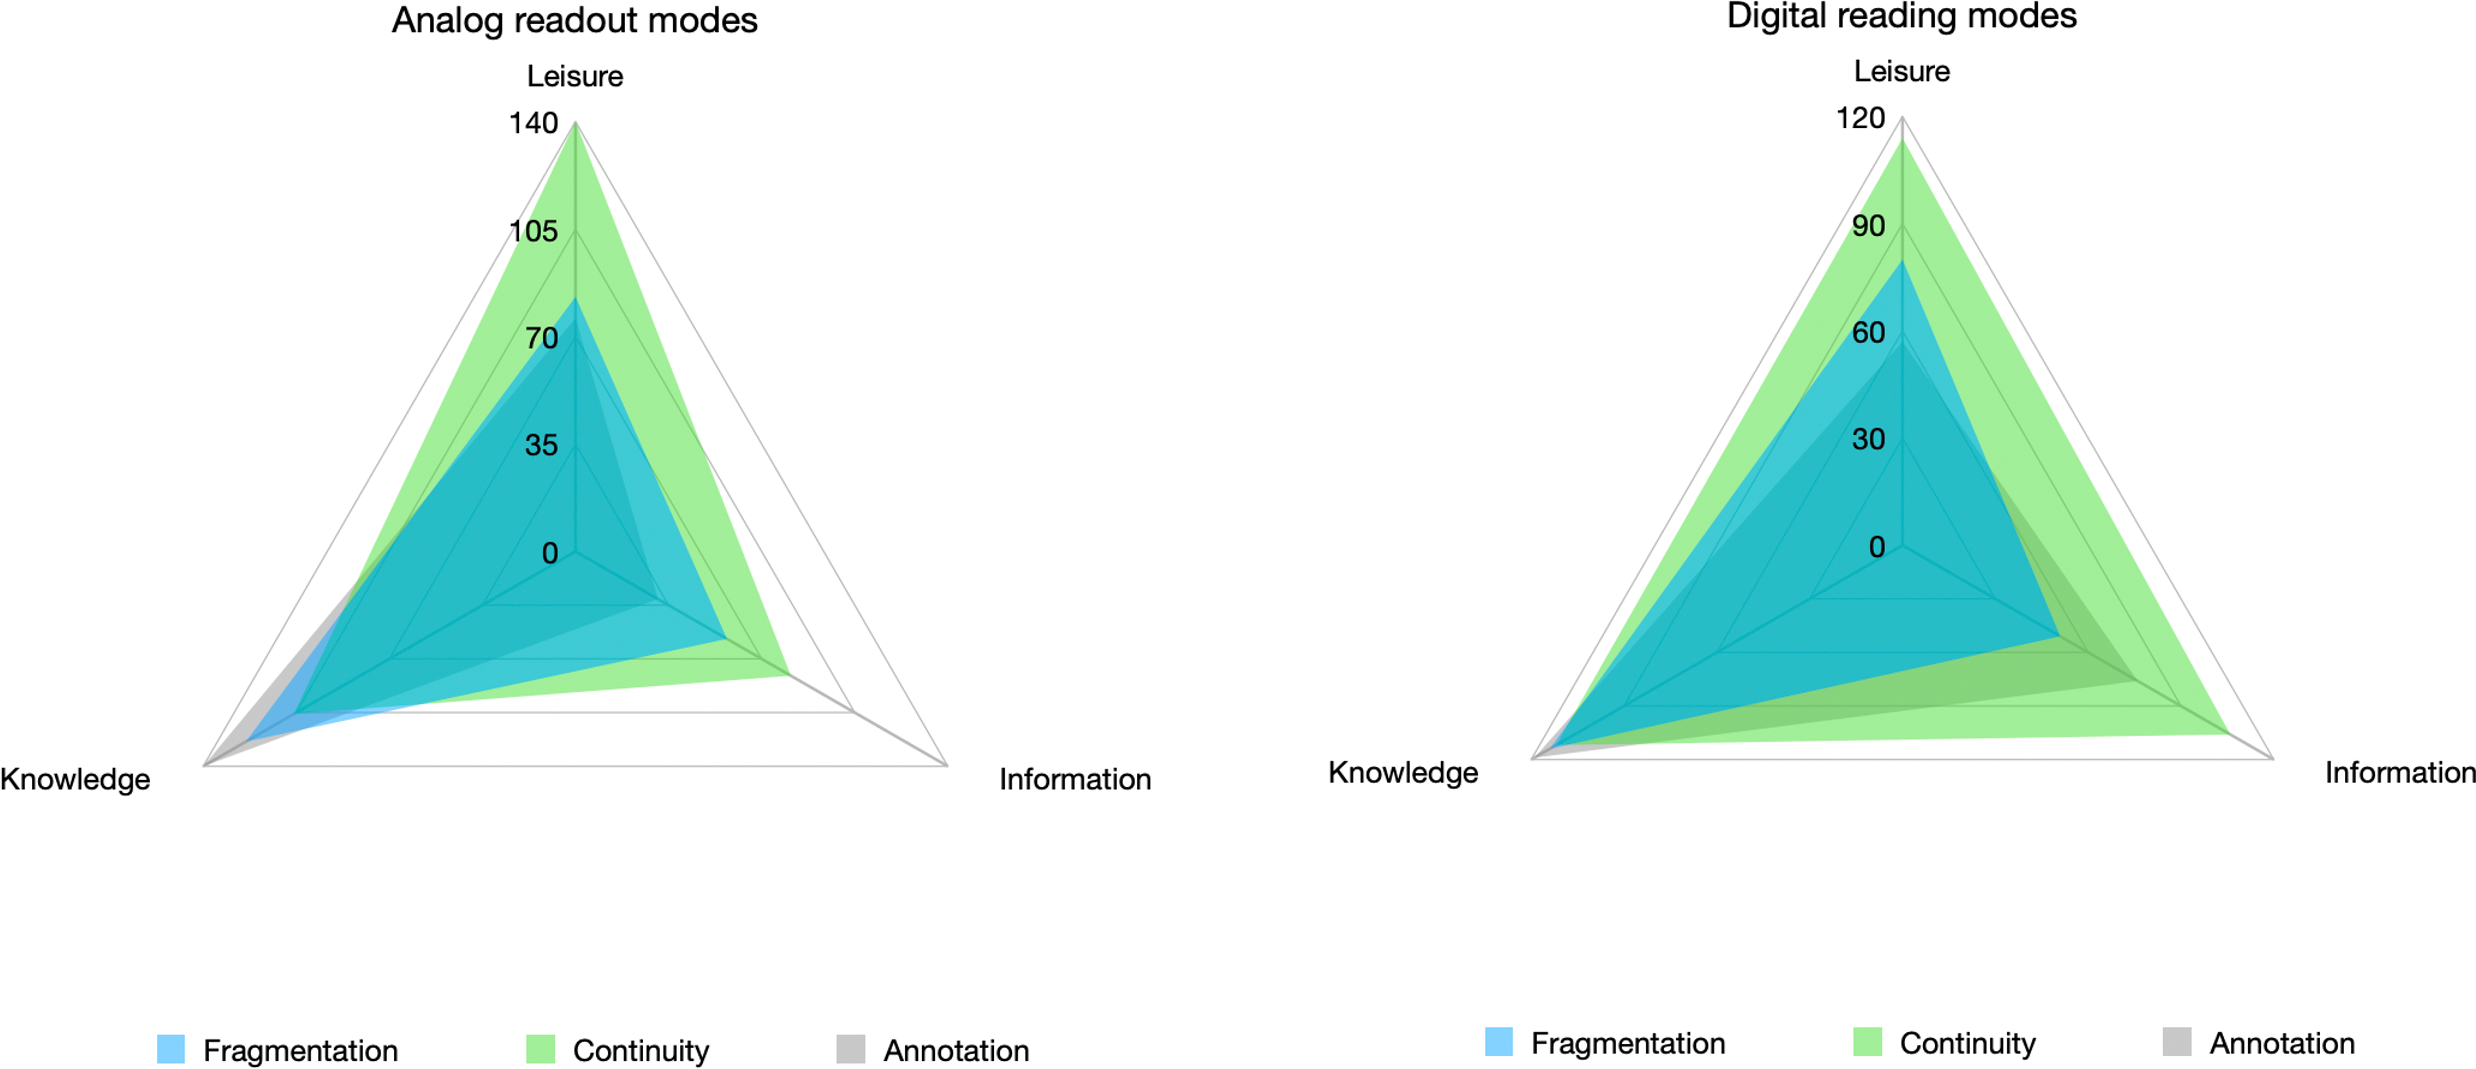
\includegraphics[width=\textwidth]{figura01.png}
 \caption{Analog and digital reading modes.}
 \label{fig01}
 \source{Own elaboration (2022).}
 \end{minipage}
\end{figure}

\subsubsection{Fragmentation}
%\emph{Fragmentation}\\
Digital readings are characterized, following \posscite{deleuze_capitalisme_1972} principle of connection and heterogeneity, by fragmentariness and fragmentation. Both from the perspective of how we read (protected by the law of mobility and ubiquity) and what we read (the special configuration of the format that leads us to microfragment the information, to facilitate access to it). Non-fragmentation of reading prevails in the three areas studied: leisure, informative and academic, at least in terms of the refusal to do so. If we pay closer attention to the extracted data, we see that fragmentation is no longer directly related to digital reading, but is extrapolated to print. The results bring us closer to similar data. This fact, like the previous ones mentioned, points to a homogenization of the reading process beyond the chosen format (\Cref{tab06} and \Cref{tab07}).


\begin{table}[h!]
\centering
\begin{threeparttable}
\caption{Analog readout modes}
\begin{tabular}{llll}
\toprule
Typology / Variable & Fragmentation & Continuity & Annotation \\
\midrule
Leisure & 83 & 140 & 76 \\
Information & 57 & 81 & 31 \\
Knowledge & 124 & 106 & 140 \\
\bottomrule
\end{tabular}
\label{tab06}
\source{Own elaboration (2022)}
\end{threeparttable}
\end{table}

\begin{table}[h!]
\centering
\begin{threeparttable}
\caption{Digital reading modes}
\begin{tabular}{llll}
\toprule
Typology / Variable & Fragmentation & Continuity & Annotation \\
\midrule
Leisure & 80 & 114 & 57 \\
Information & 51 & 106 & 76 \\
Knowledge & 114 & 112 & 119 \\
\bottomrule
\end{tabular}
\label{tab07}
\source{Own elaboration (2022)}
\end{threeparttable}
\end{table}

\subsubsection{Continuity}
%\emph{Continuity} \\ 
Some disagreement is observed with respect to the variable continuity in reading, both in leisure and information, but not in knowledge, where we have similar amounts. In the leisure and information levels, there is a lower tendency to reading continuity (\Cref{tab05} and \Cref{tab06}). The reading process, when conceived as a pastime, entails greater relaxation and less effort, which leads to discontinuity in reading. However, when dealing with academic subjects and feeling that reading is compulsory for acquiring certain knowledge, a mental process is activated that implies greater concentration and, therefore, a non-fractioned linearity.

\subsubsection{Annotation}
%\emph{Annotation} \\
Although the work of commenting on what has been read by means of quotations or annotations is used almost equally in both formats, we still find some dissimilarity that affects the digital sphere, placing it below the analogical one. Annotation prevails in both formats in readings related to knowledge, while those related to entertainment and information are lower. \\

\subsection{Preferences for use of analog and digital formats}
We now turn to the analysis of preferences in the use of a given format in the reading process (\Cref{tab08}). It is interesting to pay attention to the highest percentages, since they are the ones that reinforce the firm assertion of the choice of digital or analog. 

The preference for the printed format is maintained in formal academic tasks such as taking exams, using grammars or dictionaries and notes (more than 70 subjects out of the 185 surveyed). This last data represents a clear contradiction with the consumption analyzed above. The data on the frequency of analog format consumption show that more than three quarters of the participants state that they never or almost never use dictionaries, grammars or encyclopedias in analog format, although they claim to prefer it for these items. It is clear, therefore, that the qualities ascribed to Generation Z \cite{perez2016competencia, espiritusanto2016} prevail, those that lead them to seek a quick and immediate response, obviating preference.


\begin{table}[h!]
\centering
\begin{threeparttable}
\caption{Format preferences}
\begin{tabular}{lllllll}
\toprule
Typology & \multicolumn{2}{l}{Digital} & \multicolumn{2}{l}{Printed} & \multicolumn{2}{l}{Both} \\
 & n & \% & n & \% & n & \% \\
\midrule
RR. 			SS. & 167 & 90 & 0 & 0 & 18 & 9.7 \\
Academic 			journals & 69 & 37.29 & 27 & 16.75 & 89 & 48.1 \\
Leisure 			magazines & 56 & 30.27 & 39 & 21.08 & 90 & 48.64 \\
Academic 			forums & 130 & 70.27 & 14 & 7.56 & 41 & 22.16 \\
Leisure 			forums & 117 & 63.24 & 11 & 5.94 & 57 & 30.81 \\
Personal 			messages & 140 & 75.67 & 7 & 3.78 & 38 & 20.54 \\
Institutional 		information & 77 & 41.62 & 37 & 20 & 71 & 38.37 \\
Academic 			messages & 94 & 50.81 & 28 & 15.13 & 63 & 34.04 \\
Notes & 13 & 7.02 & 87 & 47.02 & 85 & 45.94 \\
Examinations & 8 & 4.32 & 110 & 59.45 & 67 & 36.21 \\
Grammars & 34 & 18.37 & 74 & 40 & 77 & 41.62 \\
Dictionaries & 73 & 39.45 & 31 & 16.75 & 81 & 43.24 \\
Encyclopedias & 79 & 42.70 & 34 & 18.37 & 72 & 38.91 \\
Literature 			(novel) & 15 & 8.10 & 124 & 67.02 & 46 & 24.86 \\
Literature 			(short fiction) & 17 & 9.18 & 121 & 65.4 & 47 & 25.40 \\
Academic 			books & 28 & 15.13 & 88 & 47.56 & 69 & 37.29 \\
Press & 61 & 32.9 & 32 & 17.29 & 92 & 49.72 \\
\bottomrule
\end{tabular}
\label{tab08}
\source{Own elaboration (2022)}
\end{threeparttable}
\end{table}


The high choice of the printed format for exams stands out, almost 60\%. It is true that almost 37\% of the subjects opt for indifference when taking the exams, selecting the option of both formats. We believe that the impact of Covid-19 and the obligatory digitalization of educational processes \cite{cabero2020covid, suarez-guerrero_digitalizacion_2022, ramos_ensenanza_2022} have been the main culprits of this clear rise of the digital versus the analogical in the aforementioned activities. The parallelism is also observed in the use of grammars (74 subjects versus 77), printed notes (87 versus 85 subjects) and both, respectively. It is therefore clear that the changes in sociocultural behaviors under the protection of the Internet \cite{buendia2016redes} are being extrapolated to the academic-educational environment, closer to the print-analogical, until the arrival of the pandemic. This change is equally significant in the use and reading of academic journals, with digital format or both prevailing with an almost absolute superiority, relegating the choice of printed text to barely 17\%. Reading, as already noted, is increasingly conceived as a digital process, both for leisure and for education, at least as far as the periodical press is concerned.

In the sending and receiving of messaging, as we have already pointed out, digitalization prevails, both personally and institutionally, supported by the intrinsic nature of technology that enables speed and simplicity in the communicative processes, as well as the use of different semantic languages that contribute to increase the significance of what is transmitted. 


\section{Conclusions}
The data extracted from this research show a reading habit and consumption encouraged by new technologies and digital formats. If previous research \cite{alvarez2019generacion, tabernero_sala_habitos_2020} showed how there were still certain environments where the analog format prevailed and the preference for written material still prevailed, the current data show that the border between one and the other is progressively blurring. \posscite{mcluhan_gutenberg_1962} premonition of the end of the Gutenberg era in favor of digitalization and the invasion of the screen to the detriment of the book no longer seems so distant. The gradual adaptation and constant contact with the digital world of the new generations in general and, in particular, of the Zs is leading to a change in the perception and dimension of the act of reading. Although the predilection for print is maintained in certain contexts, all of them located in the academic world, a permeability to digital format is observed, promoted and acquired by the use and constant social interaction with technology. The fragmentary reading processes typical of the digital world are also beginning to stabilize, achieving a much more continuous reading nearly similar to the analogical one. An almost total digitalization is expected in future generations, accompanied by a change in the way of facing the reading process, which will no longer be so influenced by the possible comparison with print. 

\section{Funding}
This research has been carried out within the framework of the I+D+i project PID2021-126392OB-100 “Lecturas no ficcionales para la integración de ciudadanas y ciudadanos críticos en el nuevo ecosistema cultural” [Non-fictional readings for the integration of critical citizens in the new cultural ecosystem], and the proyect “Fractales. Estrategias para la fragmentación en la narrativa española del siglo XXI” [Fractals. Strategies for fragmentation in the Spanish narrative of the XXI century] (PID2019-104215 GB-I00), funded by the Ministry of Science and Innovation. 



\printbibliography\label{sec-bib}
% if the text is not in Portuguese, it might be necessary to use the code below instead to print the correct ABNT abbreviations [s.n.], [s.l.]
%\begin{portuguese}
%\printbibliography[title={Bibliography}]
%\end{portuguese}


%full list: conceptualization,datacuration,formalanalysis,funding,investigation,methodology,projadm,resources,software,supervision,validation,visualization,writing,review
\begin{contributors}[sec-contributors]
\authorcontribution{Eva Álvarez Ramos}[conceptualization,writing]
\authorcontribution{Belén Mateos Blanco}[conceptualization,writing]
\authorcontribution{Leyre Alejaldre}[conceptualization,writing]
\end{contributors}

\end{document}

